\documentclass[twoside,11pt]{article}
\usepackage{jmlr2e}
\newcommand{\dataset}{{\cal D}}
\newcommand{\fracpartial}[2]{\frac{\partial #1}{\partial  #2}}
\ShortHeadings{95-845: AAMLP Proposal}{Gangwar, Rost and Setia}
\firstpageno{1}

\begin{document}

\title{Heinz 95-845: Project Proposal}

\author{\name Mridul Gangwar \email mgangwar@andrew.cmu.edu \\
       \addr Heinz College of Information Systems and Public Policy\\
       Carnegie Mellon University\\
       Pittsburgh, PA, United States \
       \AND
       \name Lauren Rost \email lrost@andrew.cmu.edu \\
       \addr Heinz College of Information Systems and Public Policy\\
       Carnegie Mellon University\\
       Pittsburgh, PA, United States \
       \AND
       \name Nikita Setia \email nikitas@andrew.cmu.edu \\
       \addr Heinz College of Information Systems and Public Policy\\
       Carnegie Mellon University\\
       Pittsburgh, PA, United States}
\maketitle

\section{Project Details} \label{details}

\subsection{Proposed analysis and Likely Outcomes}
This project will use a set of demographic features, usage of county-provided programs, and opioid prescription information to predict overdose deaths (opioid and non-opioid). Specifically, we propose to analyze the aforementioned data of medicaid beneficiaries from 2009 to 2017 provided by Allegheny County Department of Human Services (DHS) to predict the risk of an individual dying due to an non-opioid or opioid-related overdose. An additional component will be to clusters these individuals into groups to see if any sub-groups exist and how they relate to overdose deaths. The likely outcome of this analysis is the finding of at least one feature and subgroup that is highly deterministic in the prediction of overdose deaths, thereby enhancing the space of addiction and overdose death prevention. 

\subsection{Importance of Proposed Analysis}
National drug overdose deaths have increased over the past two decades, from 16,849 in 1999 to 70,237 in 2017 \footnote{\cite{NIDA_ODR}}. This trend is especially affected by the onset of the opioid epidemic in the late 1990s \footnote{\cite{NIDA_OOC}}. Approximately 67\% of the overdose deaths in 2017 are due to involvement of any opioids and 24\% are specifically due to prescription opioids \footnote{\cite{NIDA_ODR}}. The U.S. Department of Health and Human Services has a 5-point strategy to combat the opioid crisis \footnote{\cite{HHS}}. These points include gathering better data and conducting pertinent research to prevent addiction, thereby preventing overdose deaths. Through this analysis, we hope to contribute to the HHS strategy to combat the opioid crisis. 

\subsection{Contribution to Existing Work}
% https://jamanetwork.com/journals/jamanetworkopen/fullarticle/2728625
% Nikita to add information about fellowship and previous semester's work
% Provide references, \emph{e.g.}, see: \cite{cite1}.

\subsection{Data Description}
There are 3 datasets: demographic, DHS program activity, and opioid prescription provision containing information on 120,650 medicaid beneficiaries in Allegheny County from 2009 to 2017. The demographic data contains each person's race and gender. The program activity entails 

% Where applicable, please also define Y outcome(s), U treatment, V covariates, and W population.

\subsection{Evaluation Measures}

\subsection{Study Design, Pre-Processing and Machine Learning Methodology}

% Justify that the analysis is of appropriate size for a course project.

\subsection{Possible Study Limitations}

\subsection{Potential Future Use of Analytic Pipeline}

\bibliography{proposal_bibliography.bib}
\appendix
\section*{Appendix}

%\ref{fig:ROC_logistic}.
\begin{figure}[h]
\begin{center}
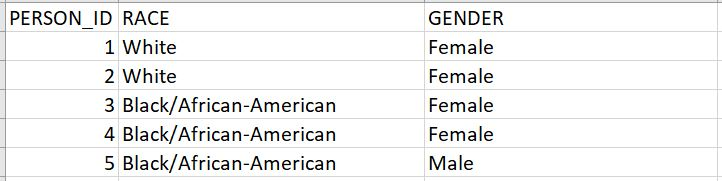
\includegraphics[width = 0.8\textwidth]{demo_head.png}
\end{center}
\caption{ROC curve for 2011 cohort prediction via GBTM's conditional probability and logistic regression; class 0 is heavy users group.}
\label{fig:ROC_logistic}
\end{figure}

\end{document}
